\documentclass[12pt,a4paper]{article}
\usepackage[utf8]{inputenc}
\usepackage[english]{babel}
\usepackage[T1]{fontenc}
\usepackage{amsmath}
\usepackage{amsfonts}
\usepackage{amssymb}
\usepackage{graphicx}
\usepackage{siunitx}
\usepackage{float}
\usepackage[left=2cm,right=2cm,top=2cm,bottom=2cm]{geometry}
\author{Gerald}

\begin{document}
\sisetup{separate-uncertainty = true}
	\setlength{\parindent}{0pt} 
	\begin{center}
		{\LARGE Experiment protocol}\\
		\begin{large}
			for the solid state lab course\\[0.4cm]
			at RWTH Aachen\\
			II. Physikalisches Institut A\\[5.5cm]
			\Large\textbf{\textsl{Quantum Transport}}\\[5.5cm]
			\normalsize\textit{authored\\by}\\[0.4cm]
			\large{Moritz Berger (355244)\\Gerald Kolter (355005)}\\[2cm]
			\large \textbf{Summer term 2019}
		\end{large}
	\end{center}
	\newpage
	
	\tableofcontents
	\newpage

\section{Introduction}
At the interfaces between different materials the fermi levels align. Therefor the conduction and valence band bend. One can use this effect to create a two dimensional electron gas ("2DEG"). This is done by building a sample of thin layers of different materials. If done correctly, the conduction band bends underneath the Fermi level in one of the layer and is above it in every other layer. \\
With this structure one builds a hall probe, meaning a rectangular sample through which a current flows from side to side. The resistivity of the sample is measured parallel and perpendicular to this current. A variable magnetic field is applied perpendicular to the 2DEG. \\
At low temperatures the density of states in the 2DEG at zero magnetic field is a simple step function. With applying a magnetic field Landau levels are formed meaning the density of states becomes a function with single peaks, whose height, width and distance to each other depend on the magnetic field. As the Fermi energy stays the same, the density of states at the Fermi energy oscillates with the magnetic field. And as the resistivity depends mainly on the density of states at the Fermi energy the resistivity parallel to the magnetic field oscillates as well. These oscillations are called "Shubnikov-de Haas oscillations". \\
The resistivity perpendicular to the magnetic field depends linearly on the magnetic field and builds Hall plateaus.


\section{Goal of the Experiment}
The goal of the experiment is to determine different properties of the 2DEG: The charge carrier concentration $n_s$, the effective electron mass $m^*$, the quantum relaxation time $\tau _q$, the transport relaxation time $\tau _{tr}$ and the effective electrons' g-factor.


\section{Setup}
The 2DEG is build between a layer of GaAs and a layer of Al$_{x}$Ga$_{1-x}$As. For applying a magnetic field an electromagnet build from a superconductor is used. For the cooling a custom build cryostat is used. It consists out of an inner liquid helium (LHe) bath in which the sample is sunk. The LHe is sunk in an outer liquid nitrogen (LN) bath. Between these two an inner vacuum insulation and around the LN an outer vacuum insulation is formed for reducing heat conductance. \\
With this setup one can cool down the sample to \SI{4.2}{K}. To reach lower temperatures one pumps the gaseous helium out of the inner tube. With this one reaches the triple point of helium at around \SI{2.2}{K}.


\section{Measurement}
The magnetic field is sweeped from \SI{-5.4}{T} to \SI{5.4}{T}. Meanwhile the resistivity parallel and perpendicular to the current is measured. This is done at without pumping, meaning at about \SI{4.2}{K}, with a fractional pumping power, meaning at about \SI{3.5}{K}, and with maximal pumping power, meaning at about \SI{2.2}{K}.

\subsection{Data}

\begin{figure} [H]
\centering
\includegraphics[scale=0.8]{Bilder/Elektron_g/4_2/Rohdaten.PNG}
\caption{Measured resistivities $R_{xx}$ and $R_{xy}$ in dependence of the magnetic field at \SI{4.2}{K}.}
\label{fig:raw_data}
\end{figure}

Fig. \ref{fig:raw_data} shows the measured raw data for the resistivities $R_{xx}$ and $R_{xy}$ in dependence of the magnetic field exemplary at \SI{4.2}{K}. The measurements at \SI{3.5}{K} and \SI{2.2}{K} yield similar results.



\section{Charge carrier concentration}
\subsection{Data analysis}


\subsection{Results}


\section{Effective electron mass}
\subsection{Data analysis}


\subsection{Results}



\section{Quantum relaxation time}
\subsection{Data analysis}


\subsection{Results}



\section{Transport relaxation time}
\subsection{Data analysis}

\subsection{Results}



\section{Electrons effective g-factor}
\subsection{Data analysis}
The resistivity of the minima of the Shubnikov-de Haas oscillation follows an Arrhenius law:
\begin{equation*}
\sigma _{xx} = \sigma _0 \cdot e^{- \frac{\Delta _{xx}}{2 k_B T}} \qquad \Leftrightarrow \qquad R _{xx} = R _0 \cdot e^{\frac{\Delta _{xx}}{2 k_B T}}
\end{equation*}
One can reformulate that to:
\begin{equation*}
\ln (R _{xx}) = \dfrac{\Delta _{xx}}{2 k_B T} + \ln (R _{0})
\end{equation*}
If the filling factor of the Hall probe is odd, the activation energy $\frac{\Delta _{xx}}{2}$ equals the Zeeman energy $g^* \mu _B B$ and so one gets:
\begin{equation*}
\ln (R _{xx}) = g^* \cdot \dfrac{\mu _B B}{k_B T} + \ln (R _{0})
\end{equation*}
Obviously one can determine the electrons effective g-factor as slope if one plots $\ln (R _{xx})$ on the y-axis and $\frac{\mu _B B}{k_B T}$ on the x-axis. \\
To extract the minima one determines the minima with a peak determination algorithm. With this one determines the B-field and the resistivity of the minimum as mean value of all datapoints which differ less than \SI{15}{\Omega} from the peak. The error is determined as the standard deviation of these datapoints. \\
This analysis is done with each measurement once with the part with positive magnetic field and once with the part with negative magnetic field.


\subsection{Results}

\begin{figure} [H]
\centering
\includegraphics[scale=0.8]{Bilder/Elektron_g/4_2/lin_fit_Arrhenius_law_1.PNG}
\caption{Linear fit of the data to the Arrhenius law exemplary for the measurement at \SI{4.2}{K} and the part with positive sign.}
\label{fig:g-factor_lin_fit}
\end{figure}

Fig. \ref{fig:g-factor_lin_fit} shows exemplary the linear fit of the data to the Arrhenius law for the part with positive magnetic field of the measurement at \SI{4.2}{K}.

\begin{table} [H]
\centering
\begin{tabular}{|c|c|c|}
\hline 
measurement at & positive sign & negative sign \\ 
\hline 
\SI{4.2 \pm 0.01}{K} & 3.44 $\pm$ 0.23 & 5.14 $\pm$ 0.37 \\ 
\hline 
\SI{3.38 \pm 0.17}{K} & 3.19 $\pm$ 0.24 & 4.09 $\pm$ 0.14 \\ 
\hline 
\SI{2.329 \pm 0.087}{K} & 3.74 $\pm$ 0.22 & 3.87 $\pm$ 0.27 \\ 
\hline 
\end{tabular} 
\caption{Measured values for the effective electrons g-factor.}
\label{tab:electron_g_factor}
\end{table}

Tab. \ref{tab:electron_g_factor} lists all determined values for the effective electrons g-factor. As one averages these one gets as result:
\begin{equation*}
g^*_{measured} = 3.85 \pm 0.20
\end{equation*}\\
\\
The theoretical value for the electrons g factor is $g_{theo} \approx 2.002$, which means the measured value for the effective g-factor differs by approximately $9.25 \, \sigma$ from the literature value. Interestingly the measured value is about twice the value from the literature. 



\section{Conclusion}



\newpage
\section*{A. Appendix}
\subsection*{Raw data}

\begin{figure} [H]
\centering
\includegraphics[scale=0.8]{Bilder/Elektron_g/2_2/Rohdaten.PNG}
\caption{Measured resistivities $R_{xx}$ and $R_{xy}$ in dependence of the magnetic field at \SI{2.2}{K}.}
\end{figure}

\begin{figure} [H]
\centering
\includegraphics[scale=0.8]{Bilder/Elektron_g/3_6/Rohdaten.PNG}
\caption{Measured resistivities $R_{xx}$ and $R_{xy}$ in dependence of the magnetic field at \SI{3.4}{K}.}
\end{figure}

\begin{figure} [H]
\centering
\includegraphics[scale=0.8]{Bilder/Elektron_g/4_2/Rohdaten.PNG}
\caption{Measured resistivities $R_{xx}$ and $R_{xy}$ in dependence of the magnetic field at \SI{4.2}{K}.}
\end{figure}

\newpage
\subsection*{Charge carrier concentration}

\newpage
\subsection*{Effective electron mass}

\newpage
\subsection*{Quantum relaxation time}

\newpage
\subsection*{Transport relaxation time}

\newpage
\subsection*{Electrons effective f-factor}

\begin{figure} [H]
\centering
\includegraphics[scale=0.5]{Bilder/Elektron_g/4_2/lin_fit_Arrhenius_law_1.PNG}
\includegraphics[scale=0.5]{Bilder/Elektron_g/4_2/lin_fit_Arrhenius_law_2.PNG}
\caption{Linear fit of the data to the Arrhenius law for the measurement at \SI{2.2}{K}.}
\end{figure}

\begin{figure} [H]
\centering
\includegraphics[scale=0.5]{Bilder/Elektron_g/3_6/lin_fit_Arrhenius_law_1.PNG}
\includegraphics[scale=0.5]{Bilder/Elektron_g/3_6/lin_fit_Arrhenius_law_2.PNG}
\caption{Linear fit of the data to the Arrhenius law for the measurement at \SI{3.4}{K}.}
\end{figure}

\begin{figure} [H]
\centering
\includegraphics[scale=0.5]{Bilder/Elektron_g/4_2/lin_fit_Arrhenius_law_1.PNG}
\includegraphics[scale=0.5]{Bilder/Elektron_g/4_2/lin_fit_Arrhenius_law_2.PNG}
\caption{Linear fit of the data to the Arrhenius law for the measurement at \SI{4.2}{K}.}
\end{figure}









\end{document}